\documentclass[a4paper,english]{article}
\usepackage{graphicx}
\usepackage{listings}
\usepackage{amsmath}
\usepackage{multirow}

%% Use utf-8 encoding for foreign characters
%%\usepackage[T1]{fontenc}
%%\usepackage[utf8]{inputenc}
%%\usepackage{babel}
%%
%%%% Vector based fonts instead of bitmaps
%%\usepackage{lmodern}
%%
%%%% Useful
%%%\usepackage{fullpage} % Smaller margins
%%\usepackage{enumerate}
%%
%%%% Theorem
%%\usepackage{amsthm}
%%
%%%% More math
%%\usepackage{amsmath}
%%\usepackage{amssymb}
\lstset{
  breaklines=true,
  postbreak=\mbox{{$\hookrightarrow$}\space},
}

%% Document Header
\title{Section1}
\author{Elliott Ashby}
\date{\today}

\begin{document}
    \maketitle
    \section{q1}
    The while loop multiplies fac by i returning it to itself then prints fac and i then increments
    i by one until i reaches 10. Essentially printing a pattern where the right number is multiplied by the 
    number on the next row on the left to find the next number on the right side. Hence \\
    \begin{center}
        \begin{tabular}{ |c|c| }
            1 & 1 \\
            2 & 2 \\
            3 & 6 \\
            4 & 24 \\
            5 & 120 \\
            6 & 720 \\
            7 & 5040 \\
            8 & 40320 \\
            9 & 362880
        \end{tabular}
    \end{center}
    Since i reaches 10 before it is multiplied by fac the while loop ends and a row with i as 10 does not get printed.
    \section{q2}
    \lstinputlisting[language=Python]{./1_2.py}
    Here we see a some code the loops over a print statement mutating the variable i each time, starting from 1 and going to 10.
    The print statement print the value, it's square and it's cube.
    \section{q3}
    The answers are m and 3 since the 4th letter of the 3rd to last element of the list b is m and the first entry in a is 3.
    \section{q4} 
    $1e^{3}$ will take a short time but is less accurate than $1e^{26}$, but $1e^{26}$ takes a long time. $1e^{7}$ is accurate enought while being still relatively fast.
    \section{q5}
    \lstinputlisting[language=Python]{./1_5.py}
    Here we simply create a list of numbers from 0 to $4\pi$ in steps of 0.01 and calculate g(x) for each of them.
    We then plot the list of x values against the list of g(x) values adding axis labels and tick names.
    \begin{center}
        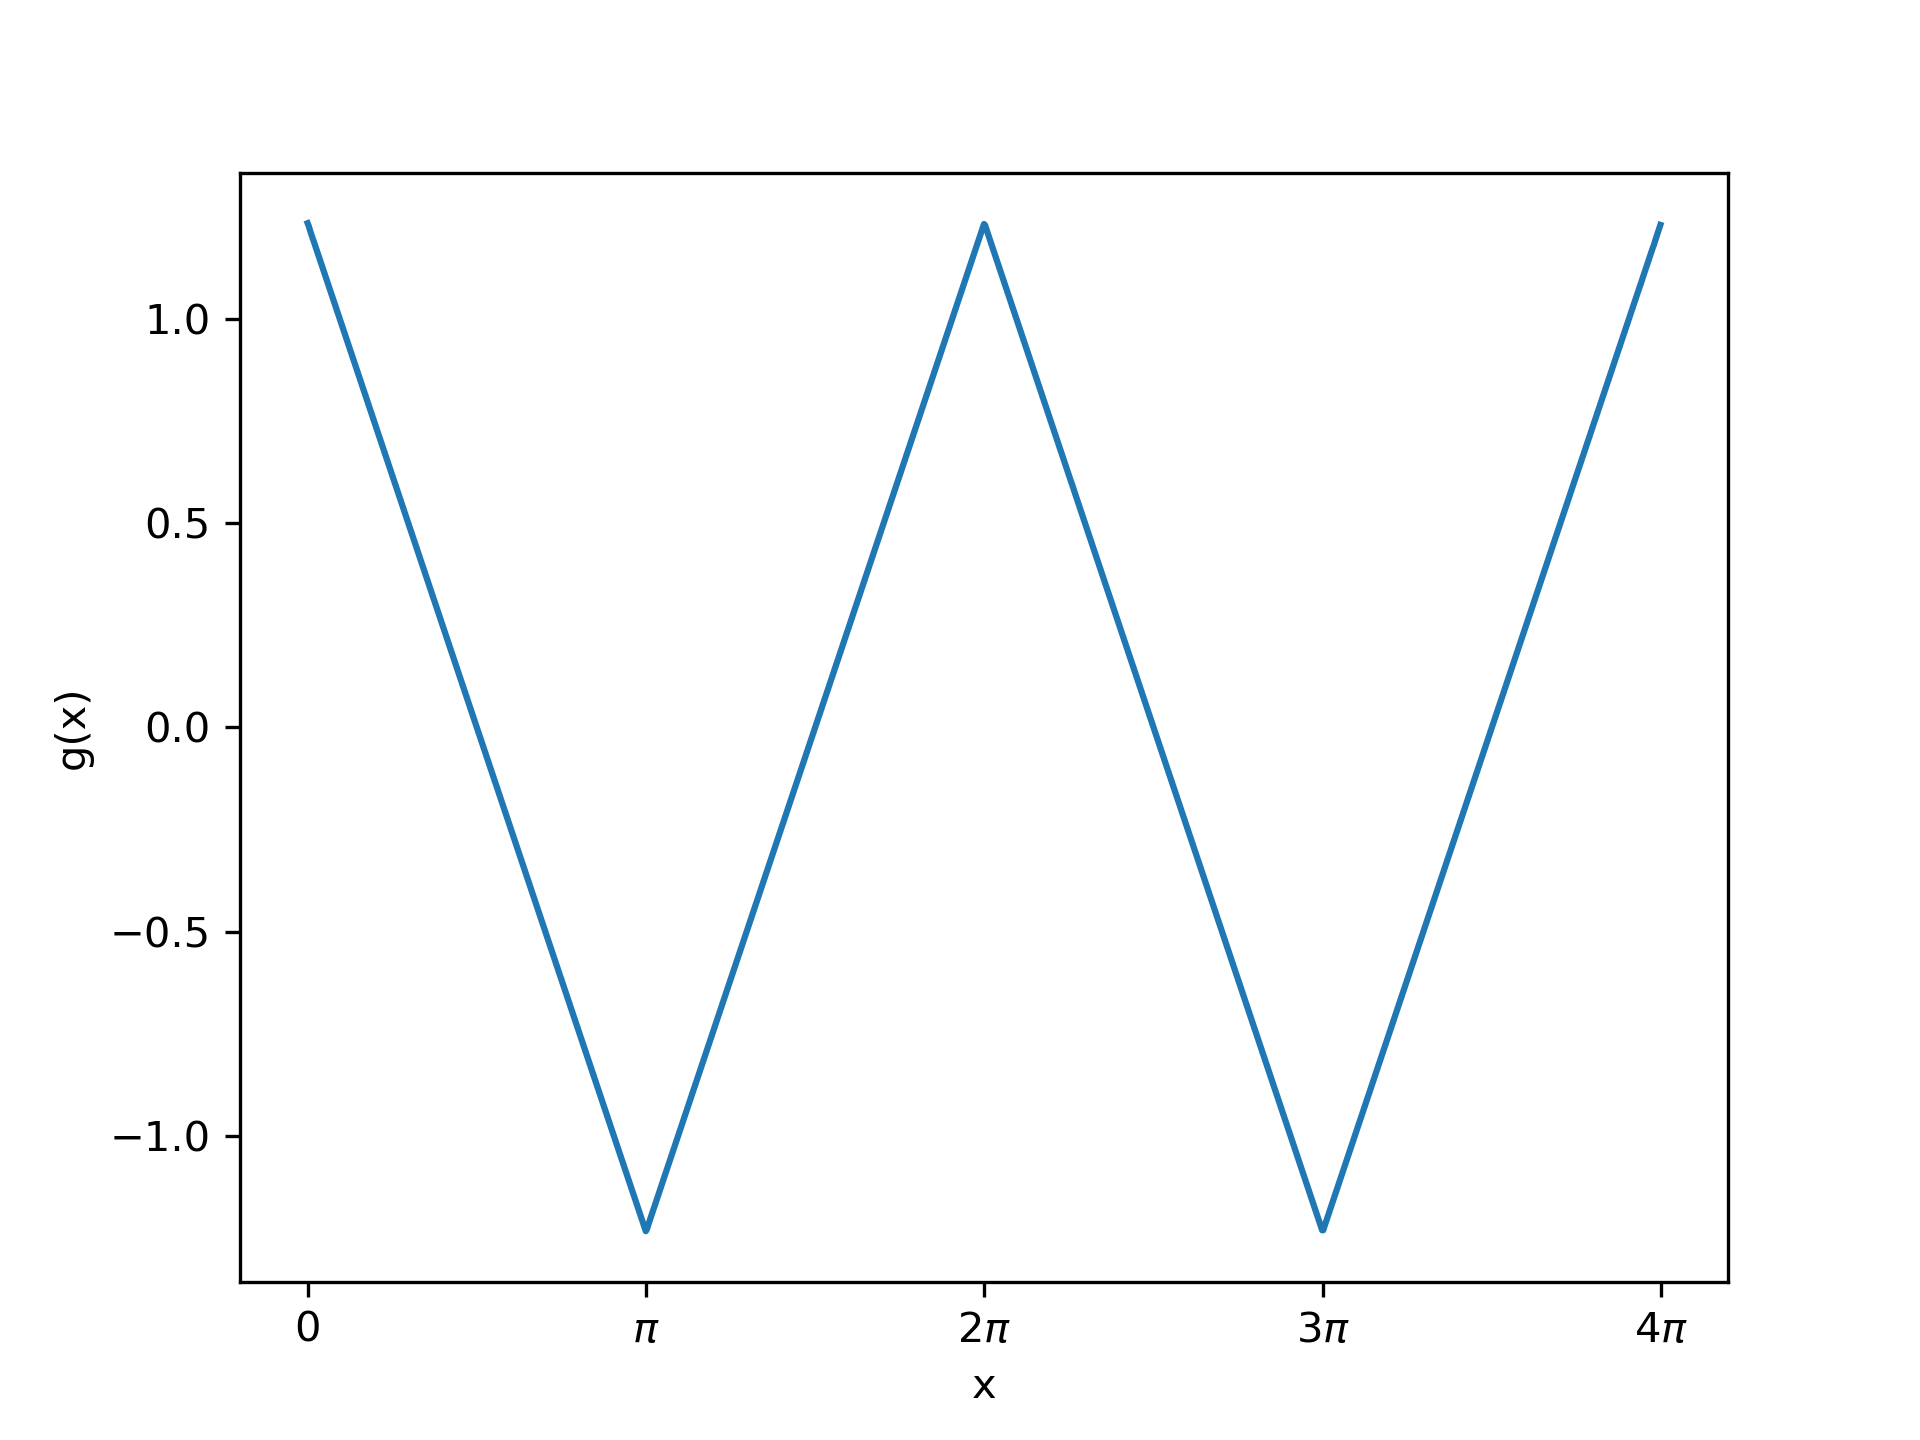
\includegraphics[scale=0.8]{./1_5.png}
    \end{center}
    \section{q6}
    \lstinputlisting[language=Python]{./1_6.py}
    We start by defining our constants, samplesm range and number of bins, we the create the binned data by calling the sort to bins function and the gen data function inside that.
    We then plot the data as a bar graph with the x axis being the bins and the y axis being the number of samples in each bin.
    \begin{center}
        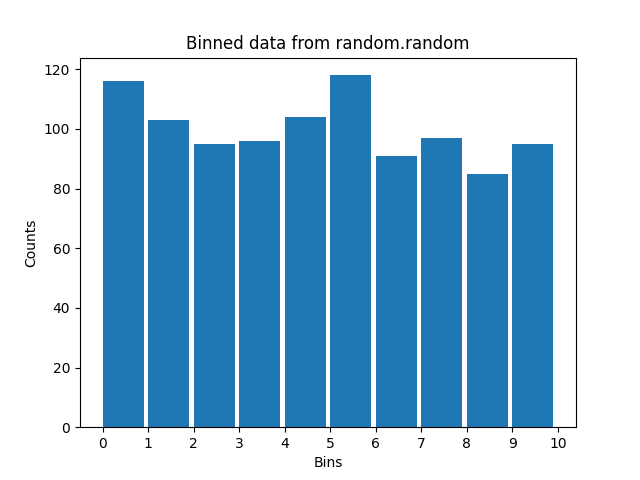
\includegraphics[scale=0.8]{./1_6.png}
    \end{center}
    \section{q7}
    \lstinputlisting[language=Python]{./1_7.py}
    Therefore:
    \begin{center}
        $4.53988$\% are outside of the range $-2 < x < 2$
    \end{center}
    With obviously some variation in percentage calcuated, however to minimise this the code is ran "repeats" number of times and an average is found.
    \section{q8}
    \lstinputlisting[language=Python]{./1_8.py}
    Here we change the code given to us from a set number of runs "n" to a stopping condition, in this case I chose $1e^{-7}$ since it resulted in a reasonable amount of precision.
    Here we output the result as:
    \begin{center}
        1051.2492201029809
    \end{center}
\end{document}
